\PassOptionsToPackage{table,dvipsnames,svgnames}{xcolor}
\documentclass[a4paper,10pt]{article}

% === Encoding & Sprache ===
\usepackage[T1]{fontenc}
\usepackage[utf8]{inputenc}
\usepackage[english]{babel}
\usepackage{newunicodechar}
\usepackage{comment}
\newunicodechar{−}{-}


% === Schrift ===
\usepackage{helvet} % Helvetica verfügbar
\renewcommand{\familydefault}{\sfdefault} % sans-serif font type (in printed versions serif is easier to read, in digital form sans-serif is easier to read)

% === Mathematik & Chemie ===
\usepackage{amsmath,amssymb,bm}
\usepackage{chemformula}

% === Seitenlayout ===
\usepackage[left=2cm,right=2cm,top=2.8cm,bottom=2.8cm]{geometry}
\usepackage{rotating}

% === Tabellen & Spalten ===
\usepackage{array}
\usepackage{tabularx}
\usepackage{caption} % put in preamble
\usepackage{capt-of}
\usepackage{booktabs}
\usepackage{longtable}
\usepackage{multirow}
\usepackage{threeparttable}
\newcolumntype{Y}{>{\centering\arraybackslash}X}
% Flexible Spalten (einheitliche L-Definition)
\newcolumntype{L}[1]{>{\RaggedRight\arraybackslash\hspace{0pt}}p{\dimexpr#1-2\tabcolsep\relax}}

% === Grafiken & Abbildungen ===
\usepackage{graphicx}
\usepackage{adjustbox}
\usepackage{wrapfig}
\usepackage{sidecap}
\usepackage{svg}
\usepackage{tikz}
\usepackage{subcaption}
\usepackage{pdflscape}
\usepackage{url}
\usepackage{pdfpages}

% === Farben (cleaned version) ===
\usepackage{xcolor} % core color package
\usepackage{xkcdcolors}                        % optional xkcd color palette

% --- Custom ESA / project colors ---
\definecolor{ESAblue}{RGB}{0,56,168}
\definecolor{ESAgreen}{RGB}{0,150,0}
\definecolor{ESAred}{RGB}{200,0,0}
\definecolor{hummocky}{RGB}{79,189,255}
\definecolor{mottled}{RGB}{255,179,0}
\definecolor{angular}{RGB}{157,60,255}
\definecolor{powder}{RGB}{255,68,171}
\definecolor{Bennu}{RGB}{0,0,255}
\definecolor{Poster}{RGB}{55,55,255}
\definecolor{Perseuss}{RGB}{46,139,87}
\definecolor{perseuss}{RGB}{80,200,120}
\definecolor{headbg}{HTML}{F0F3F7}
\definecolor{bandbg}{HTML}{FAFAFA}
\definecolor{Laser}{RGB}{136,193,74}
\definecolor{LASERfinal}{RGB}{82,186,158}

% --- Optional standard colors to avoid undefined errors ---
% These define safe, capitalized versions in case any package or comment uses them
\definecolor{RED}{named}{red}
\definecolor{GREEN}{named}{green}
\definecolor{BLUE}{named}{blue}
\definecolor{BLACK}{named}{black}

% --- Cell header command for tables ---
\newcommand{\thdr}[1]{\cellcolor{headbg}\textbf{#1}}


% === Beschriftungen ===
\usepackage{caption}
\captionsetup{font=small}
\captionsetup[figure]{labelfont={bf},name={Fig.},labelsep=period}
\captionsetup[table]{labelfont={bf},name={Table},labelsep=period}
\captionsetup[subfigure]{width=0.9\textwidth}

% === Einheiten & Symbole ===
\usepackage{siunitx}
\DeclareSIUnit\year{a}
\usepackage{gensymb}
\usepackage{wasysym}
\usepackage{textcomp}

% === Verweise & Literatur ===
% === Verweise & Literatur ===
\usepackage[numbers,square]{natbib}
\usepackage[nottoc]{tocbibind}
\usepackage[colorlinks,bookmarks=false,linkcolor=purple,
            urlcolor=blue,citecolor=purple]{hyperref}
\usepackage{cleveref}
\crefname{table}{Table}{Tables}
\crefname{section}{Section}{Sections}
\crefname{figure}{Fig.}{Figs.}
\crefname{equation}{Eq.}{Eqs.}
\Crefname{figure}{Figure}{Figures}




% === Anhänge ===
\usepackage[titletoc]{appendix}

% === Listen, Floats, Satz ===
\usepackage{enumitem}
\usepackage{float}
\usepackage{ragged2e}
\usepackage{parskip}
\setlength{\parindent}{1cm}
\usepackage{setspace}
\setstretch{1.25}
\usepackage[normalem]{ulem}
\usepackage{lipsum}

% === Abschnittstitel & Boxen ===
\usepackage[explicit]{titlesec}
\usepackage{tcolorbox}
% --- Define box styles ---
\tcbset{
  bluetitle/.style={
    enhanced,
    colback=perseuss,
    colframe=white,
    boxrule=0.5pt,
    width=\textwidth,
    left=6pt, right=6pt, top=4pt, bottom=0pt,
    arc=2pt,
    boxsep=0pt,
    enlarge bottom by=-10pt
  },
  chaptertitle/.style={
    enhanced,
    colback=Perseuss,
    colframe=white,
    boxrule=0.5pt,
    width=\textwidth,
    left=6pt, right=6pt, top=4pt, bottom=0pt,
    arc=2pt,
    boxsep=0pt,
    enlarge bottom by=-10pt
  },
  whitesubtitle/.style={
    enhanced,
    colback=white,
    colframe=blue!50!black,
    boxrule=0.5pt,
    width=\textwidth,
    left=6pt, right=6pt, top=3pt, bottom=3pt,
    arc=0pt,
    boxsep=0pt,
    enlarge top by=-0.5pt
  }
}

% === Kopf- und Fußzeilen ===
\usepackage{fancyhdr}
\pagestyle{fancy}
\fancyhead{}
\fancyfoot[LO,RE]{}
\fancyfoot[LE,RO]{}
\fancyhead[LE,RO]{FS26}
\fancyhead[C]{}
\fancyhead[LO,RE]{Space Data Project 3}
\fancyfoot[C]{\thepage}

% === Zähler & Tiefen ===
\setcounter{secnumdepth}{4}
\setcounter{tocdepth}{4}

% === Absatzformatierung ===
\makeatletter
\renewcommand\paragraph{\@startsection{paragraph}{4}{\z@}%
  {3ex plus .2ex minus 0ex}{1ex}%
  {\normalfont\normalsize\bfseries}}
\makeatother

% === Doppelseitenumbruch anpassen ===
\makeatletter
\def\cleardoublepage{\clearpage\if@twoside \ifodd\c@page\else
\hbox{}
\vspace*{\fill}
\thispagestyle{empty}
\newpage
\if@twocolumn\hbox{}\newpage\fi\fi\fi}
\makeatother

% === Tabellenabstände ===
\renewcommand{\arraystretch}{1.02}
\setlength{\tabcolsep}{4pt}
\setlength{\extrarowheight}{0pt}

% === Sonstige Makros ===
\newcommand{\tbd}{\textbf{TBD}}
\newcommand{\otoprule}{\midrule[\heavyrulewidth]}
\newcommand*\rot{\rotatebox{90}}
\newcommand{\fathline}{\rule{\linewidth}{0.5mm}}
\newcommand\nobrkhyph{\mbox{-}}
\widowpenalty=9999
\clubpenalty=9999

% Farbige S-Zellen (gelassen wie vorgegeben)
\renewcommand{\S}[1]{%
  \begingroup
  \def\n{#1}%
  \ifcase\n\relax
    \cellcolor{white}\textbf{#1}%
  \or
    \cellcolor{red!70}\textbf{1}%
  \or
    \cellcolor{red!40!yellow}\textbf{2}%
  \or
    \cellcolor{yellow!65}\textbf{3}%
  \or
    \cellcolor{green!35!yellow}\textbf{4}%
  \or
    \cellcolor{green!65}\textbf{5}%
  \else
    \cellcolor{white}\textbf{#1}%
  \fi
  \endgroup
}

% ------- alternative title formatting (als Kommentar belassen) ------
\begin{comment}
\titleformat{\chapter}[display]
  {\Huge\scshape}
  {\filleft\tikz\node[fill=green!50!black!10,rectangle,rounded corners=6pt] (chap) {\chaptertitlename};}
  {0ex}
  {\colorbox{green!50!black!10}{\parbox{\dimexpr\textwidth-2\fboxsep\relax}{\vskip1ex#1\vskip1ex}}}
\end{comment}

\begin{comment}
% define some colors
\definecolor{section}{RGB}{10,221,164}
\definecolor{subsection}{RGB}{200,255,240}
\definecolor{titletext}{RGB}{0,0,0}
\definecolor{turkis}{RGB}{2,159,106}

% section color box
\setkomafont{section}{\mysection}
\newcommand{\mysection}[1]{%
	\Large\sf%
	\setlength{\fboxsep}{0cm}%
	\colorbox{section}{%
		\begin{minipage}{\linewidth}%
			\vspace*{2pt}%
			\leftskip2pt
			\rightskip\leftskip
			{\color{titletext} #1}
			\vspace*{1pt}%
		\end{minipage}%
}}

% subsection color box
\setkomafont{subsection}{\mysubsection}
\newcommand{\mysubsection}[1]{%
	\Large\sf%
	\setlength{\fboxsep}{0cm}%
	\colorbox{subsection}{%
		\begin{minipage}{\linewidth}%
			\vspace*{2pt}%
			\leftskip2pt
			\rightskip\leftskip
			{\color{titletext} #1}
			\vspace*{1pt}%
		\end{minipage}%
}}
\end{comment}

% ------------ alternative (als Kommentar belassen) ---------
\begin{comment}
\titleformat{\section}
  {\Large\rmfamily\bfseries\color{Perseuss}}{\thesection}{1em}{#1}

\titleformat{\subsection}
  {\Large\rmfamily\bfseries\color{perseuss}}{\thesection}{1em}{#1}
\end{comment}

% ------- Hinweise / alte, auskommentierte Zeilen beibehalten -------
% \usepackage[comma]{natbib}
% \usepackage{graphicx}


\begin{document}


% ====== Indentation (no stupid indentation :) ) 
\setlength{\parindent}{0pt}

% TITLE PAGE ########################
\begin{comment}
\newgeometry{top=1.5cm, bottom=1.5cm, left=2cm, right=2cm}
\begin{titlepage}
\pagenumbering{gobble} 
\thispagestyle{empty}
\noindent 
\includegraphics[scale=0.2]{Figures/Figures General/eth logo.png} 
%\hfill\includegraphics[scale=0.68]{}
\begin{singlespace}  
%\vspace{-10pt} 
\noindent 
\begin{center} 
    \includegraphics[height=13cm]{Figures/la plata basin.jpg} 
\end{center} 
%\begin{center}
%    \textbf{\LARGE{\textcolor{perseuss}{PERSEUSS\\ 
%    \rule{\linewidth}{.2pt} 
%    \large 
%    \textcolor{perseuss}{Photon-based Explorational Reconnaissance of Sublunar Environments, Underground Structures and Surfaces\\ Mission Project Analysis}}}}
%\end{center}

\begin{center}
    \textbf{ 
    \rule{\linewidth}{.4pt}\\
    \vspace{8pt}
    \large 
    \textcolor{purple}{El Niño vs La Niña Effects in the La Plata Basin}\\
    \vspace{3pt} 
    \rule{\linewidth}{.4pt}\\
    \vspace{5pt}
    \textcolor{purple}{How do El Niño and La Niña differently affect terrestrial water storage in the La Plata Basin in terms of spatial pattern and magnitude? }}
\end{center}
\vspace{25pt} 
\noindent 
\begin{minipage}[t]{0.45\textwidth} 
    \textbf{Authors:}\\ 
    Stasha Petrovikj\\
    Isabel Reinecke\\  
\end{minipage} 
\hfill 
\begin{comment}
\begin{minipage}[t]{0.45\textwidth} 
    \raggedleft 
    \textbf{Supervisors:}\\ 
    Prof. Thomas Zurbuchen\\
    Dr. Simon Stähler\\ 
    Dr. Florian Kehl\\   
\end{minipage}

\vspace{18pt} 
\noindent 
\vspace{0.5cm}
\textbf{\today}
\end{singlespace}
\vspace{40pt} 
\includegraphics[scale=0.25]{Figures/Figures General/eth space logo 2 2.png}\hfill{\includegraphics[scale=0.125]{Figures/Figures General/eaps logo.png}}

\begin{flushleft} 
    \includegraphics[scale=0.22]{Figures/Figures General/eth space logo 2 2.png} 
\end{flushleft} 
\vspace{-30pt}\centering\includegraphics[scale=0.13]{Figures/Figures General/eaps logo.png} 

\hfill\vspace{20pt}\includegraphics[scale=0.18]{Figures/Figures General/logo orb vel 2.png}


\end{titlepage}
\restoregeometry
\end{comment}
%######### MISSION SUMMARY TABLE ################



%######## AUTHORSHIP AND ACKNOWLEDGEMENTS #################

\newpage
\setstretch{1}
\begin{comment}
    

\section*{Authorship and Acknowledgments}
\thispagestyle{plain}
\subsubsection*{Team}
    Author A\\
    Author B\\
    Author C\\  

\subsection*{Acknowledgements}

\textcolor{red}{We would like to thank...}

\end{comment}
\vspace{-30pt}
\begin{center}
    \textbf{ 
    %\rule{\linewidth}{.4pt}\\
    %\vspace{8pt}
    \huge 
    \textcolor{purple}{Denoising PSRs with CNNs}\\
    %\vspace{3pt} 
    \rule{\linewidth}{.4pt}\\
    \vspace{5pt}
    \textcolor{purple}{\normalsize{Mattia De Martino - Isabel Reinecke - Marius Riesterer }}}
\end{center}


% LIST OF CONTENTS, FIGURES AND TABLES ########################

\begin{comment}
    

{\hypersetup{linkcolor=black}
\setcounter{tocdepth}{3}
\tableofcontents}


{\hypersetup{linkcolor=black}
\listoffigures}
%\newpage
%\newpage
%{\hypersetup{linkcolor=black}
%\listoftables}


 % You may want to start the first section on a new page


\end{comment}
% CHAPTERS ########################
% \input{List of Acronyms}

% start page numbering at page 1
\pagenumbering{arabic}\setcounter{page}{1}
\section{Introduction}
Denoising lunar images is essential for reliable interpretation of permanently shadowed regions, where high noise levels can hide small craters, local albedo changes, and regolith texture. In this open project, the task was to adapt the previous denoising pipeline to a harder dataset of higher-resolution, noisier lunar images. The training set contains paired noisy and clean images, while the test set contains only noisy images with clean targets held back. We therefore treated the task as supervised image-to-image regression during training, selected models using paired validation metrics, and inspected blind-test predictions qualitatively.

Starting from the Task 2 baseline, we investigated changes in architecture, capacity, optimization, loss functions, regularization, and output activation. The best model was a large four-stage Deep U-Net. It achieved the best completed validation score: MSE $=0.001758$, MAE $=0.03213$, and PSNR $=27.55$ dB.

\section{Method}
We explored several architecture families: standard U-Nets, attention-gated U-Nets, residual CNN denoisers, residual U-Nets, autoencoders, DINOv2-based feature decoders, and conditional diffusion models. U-Net-based models were especially well matched to this task because the encoder-decoder structure captures multi-scale noise patterns, while skip connections preserve high-resolution spatial details. Attention U-Nets were tested to suppress irrelevant skip features, and ResNet-style denoisers were tested as a full-resolution alternative. Diffusion models and DINOv2 decoders were included as higher-risk approaches to test whether more advanced representation learning could improve perceptual quality.

We first ran ablation studies to reduce the search space. The ablations varied feature-channel capacity, architecture depth, loss function, optimizer, learning rate, output activation, and regularization. After identifying Deep U-Nets as the strongest family, we used Optuna for hyperparameter optimization. Optuna samples configurations from a defined search space, trains each trial for a limited budget, evaluates validation PSNR, and uses pruning to stop trials whose intermediate score is unlikely to become competitive. For the Deep U-Net search, the sampled parameters included feature scale, dropout, sigmoid versus tanh output, learning rate, weight decay, optimizer, and batch size.

\subsection{Dataset and Metrics}
The dataset consists of 19\,500 paired noisy/clean lunar images of size $128\times128$ and 1\,000 blind noisy test images. Arrays were converted to \texttt{float32}, normalized to $[0,1]$ by dividing by 255 when necessary, and loaded as single-channel tensors. Final reruns used a deterministic 5\% validation split and were trained on Euler GPUs.

On paired validation data, PSNR was computed in the standard full-reference way from the MSE between the denoised output $\hat{x}$ and the clean target $x$:
\[
\mathrm{PSNR}=10\log_{10}\left(\frac{1}{\mathrm{MSE}(\hat{x},x)}\right),
\]
because images are normalized to $[0,1]$. On the blind test set, clean targets are not available, so true test MSE, MAE, or PSNR cannot be computed locally. The blind test images were therefore denoised for submission and inspected visually, while all quantitative model selection was based on paired validation data.

\subsection{Final Model Architecture}
\label{sec:model_arch}
Only the final model is shown in detailed tabular form. The selected architecture is a large four-stage Deep U-Net with feature channels $[64,128,256,512]$, a $1024$-channel bottleneck, batch normalization, ReLU activations, dropout $p=0.10887$, transposed-convolution upsampling, concatenated skip connections, and a sigmoid output.

\begin{table}[H]
\centering
\caption{Detailed architecture of the best model, a large four-stage Deep U-Net. Input and output images have shape $(1,128,128)$.}
\begin{tabular}{lllr}
\toprule
\textbf{Stage} & \textbf{Layer Name} & \textbf{Operation / Output Shape} & \textbf{Parameters} \\
\midrule
\multirow{5}{*}{Encoder}
& input & Grayscale input $(1,128,128)$ & 0 \\
& enc1 & DoubleConv $(64,128,128)$ & 37,696 \\
& enc2 & MaxPool + DoubleConv $(128,64,64)$ & 221,696 \\
& enc3 & MaxPool + DoubleConv $(256,32,32)$ & 885,760 \\
& enc4 & MaxPool + DoubleConv $(512,16,16)$ & 3,540,992 \\
\midrule
Bottleneck
& bottleneck & MaxPool + DoubleConv $(1024,8,8)$ & 14,159,872 \\
\midrule
\multirow{8}{*}{Decoder}
& up4 & ConvTranspose2D $(512,16,16)$ & 2,097,664 \\
& dec4 & Concatenate skip + DoubleConv $(512,16,16)$ & 7,079,936 \\
& up3 & ConvTranspose2D $(256,32,32)$ & 524,544 \\
& dec3 & Concatenate skip + DoubleConv $(256,32,32)$ & 1,770,496 \\
& up2 & ConvTranspose2D $(128,64,64)$ & 131,200 \\
& dec2 & Concatenate skip + DoubleConv $(128,64,64)$ & 442,880 \\
& up1 & ConvTranspose2D $(64,128,128)$ & 32,832 \\
& dec1 & Concatenate skip + DoubleConv $(64,128,128)$ & 110,848 \\
\midrule
Output
& out\_conv & $1\times1$ Conv2D + Sigmoid $(1,128,128)$ & 65 \\
\midrule
\multicolumn{3}{r}{\textbf{Total Trainable Parameters}} & \textbf{31,036,481} \\
\bottomrule
\end{tabular}
\end{table}

\subsection{Training Setup}
The final model was trained with MSE loss, AdamW, learning rate $9.664\cdot10^{-4}$, weight decay $2.472\cdot10^{-3}$, batch size 16, and a cosine learning-rate scheduler for 150 epochs. Dropout, AdamW weight decay, validation checkpointing, and the U-Net skip-connection structure were used to control overfitting. The best checkpoint was selected by validation error. For comparison, the best Attention U-Net candidates used a combined $0.5\cdot\mathrm{MSE}+0.5\cdot\mathrm{L1}$ loss and learning rates around $4\cdot10^{-4}$, while diffusion candidates used MSE loss, AdamW, and DDIM-style validation.

\section{Results}

\subsection{Ablation Results}
Throughout this project, a broad set of configurations was explored. The main ablation categories are summarized in Table~\ref{tab:ablations}. The strongest trend was architectural: deeper multi-scale U-Nets consistently outperformed flat ResNets, autoencoders, and attention-gated variants on validation MSE/PSNR. MSE was selected for the final Deep U-Net because it directly optimizes the reported pixel-wise error and PSNR. L1 or mixed losses sometimes produced visually plausible outputs, but did not improve the final validation score.

\begin{table}[H]
\centering
\small
\setlength{\aboverulesep}{2pt}
\setlength{\belowrulesep}{2pt}
\caption{Ablation studies overview. The best performing choices for the final model family are highlighted in bold.}
\label{tab:ablations}
\begin{tabular}{llp{8.5cm}}
\toprule
\textbf{Ablation Study} & \textbf{Parameter Varied} & \textbf{Candidates / Configurations} \\
\midrule
Network Capacity & Feature Channels & Small, default, and \textbf{large} feature maps; ResNet variants with 8 and 16 residual blocks \\
\midrule
Architecture & Structural Block / Gating & Standard U-Net, Attention U-Net, \textbf{Deep U-Net (4 stages)}, Res-UNet, Autoencoder, Flat ResNet, diffusion, DINOv2 decoder \\
\midrule
Loss Function & Optimization Objective & \textbf{MSE}, L1, combined MSE/L1, MS-SSIM/L1-inspired loss \\
\midrule
Optimization Setup & Optimizer \& Learning Rate & Adam and \textbf{AdamW}; Optuna-searched learning rates and weight decay \\
\midrule
Output Layer & Activation Function & \textbf{Sigmoid} vs. tanh mapped to $[0,1]$ \\
\bottomrule
\end{tabular}
\end{table}

\begin{figure}[H]
\centering
\begin{subfigure}{0.48\textwidth}
    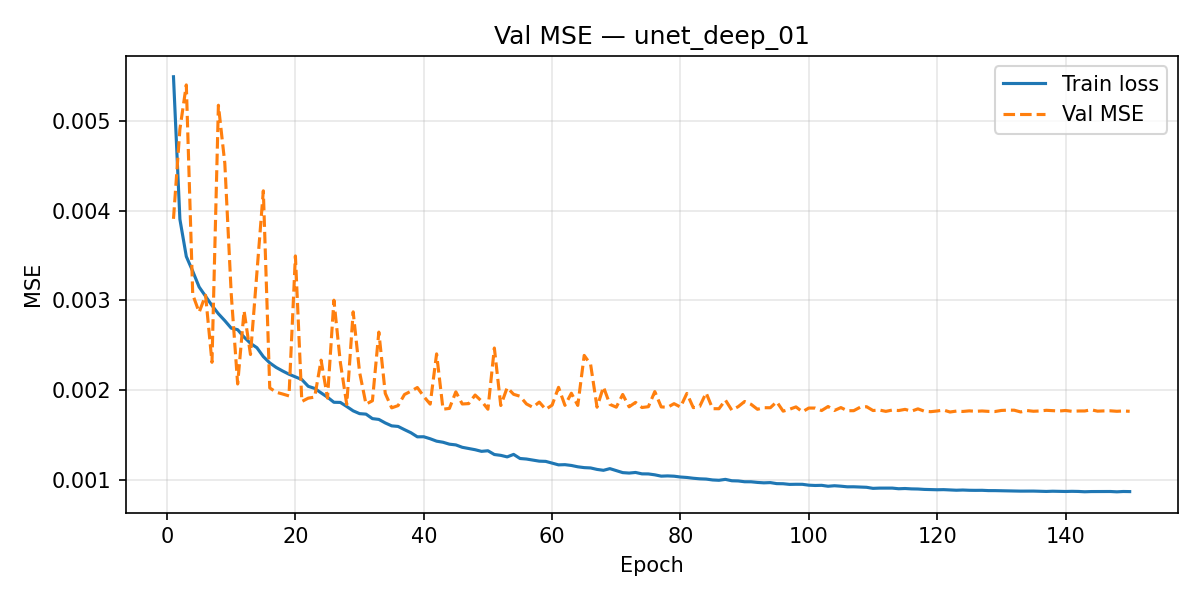
\includegraphics[width=\linewidth]{images/final_deep_unet_mse.png}
    \caption{Final Deep U-Net training loss and validation MSE.}
\end{subfigure}
\hfill
\begin{subfigure}{0.48\textwidth}
    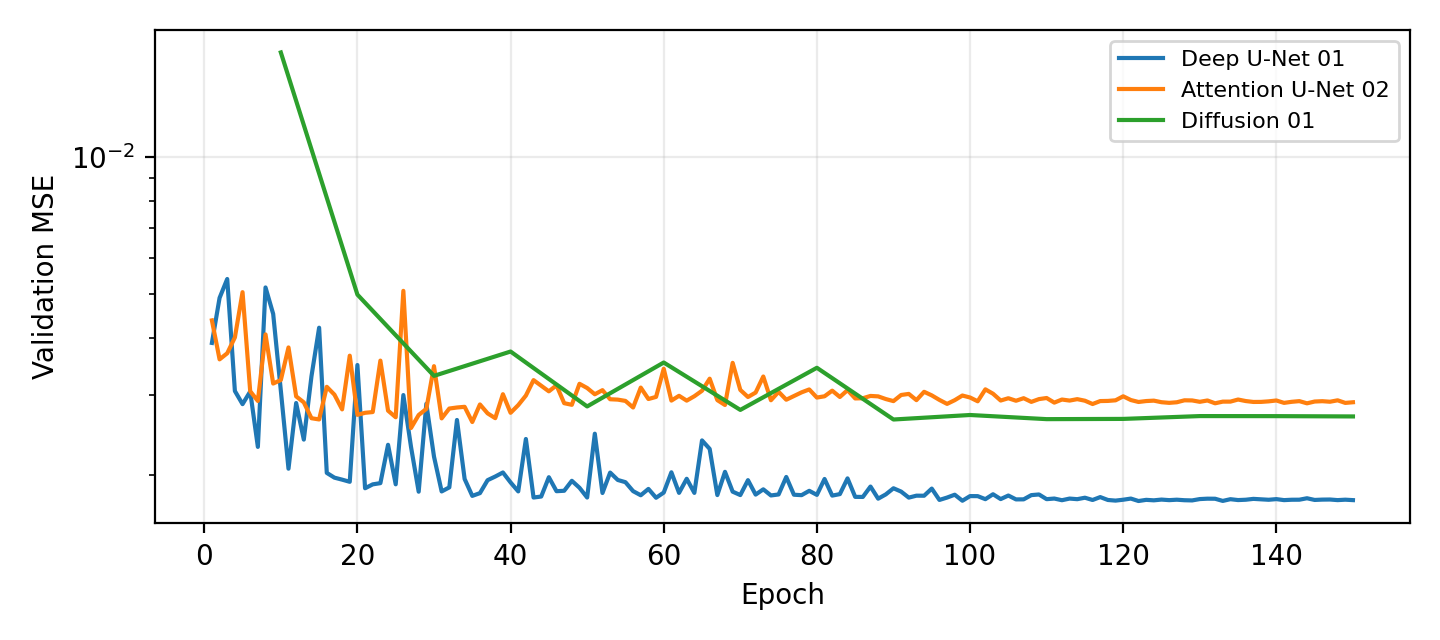
\includegraphics[width=\linewidth]{images/three_config_val_mse.png}
    \caption{Validation MSE for representative final configurations.}
\end{subfigure}
\caption{Loss curves used to assess training stability and model selection.}
\end{figure}

\subsection{Final Results}
The best model was a large four-stage Deep U-Net. It reached a best validation MSE of $0.001758$, MAE of $0.03213$, and PSNR of $27.55$ dB. A closely related Deep U-Net configuration reached PSNR $27.53$ dB, indicating that the Deep U-Net family was robust rather than a single lucky configuration.

\begin{table}[H]
\centering
\caption{Final candidate comparison on paired validation data.}
\begin{tabular}{llcc}
\toprule
Model & Main difference & Best val. MSE & Val. PSNR [dB] \\
\midrule
\textbf{Best Deep U-Net} & large 4-stage U-Net, MSE & \textbf{0.001758} & \textbf{27.55} \\
Alternative Deep U-Net & higher LR and dropout & 0.001767 & 27.53 \\
Attention U-Net & attention gates, combined loss & 0.002542 & 25.95 \\
Diffusion model & conditional DDPM-style model & 0.002654 & 25.76 \\
\bottomrule
\end{tabular}
\end{table}

\begin{figure}[H]
\centering
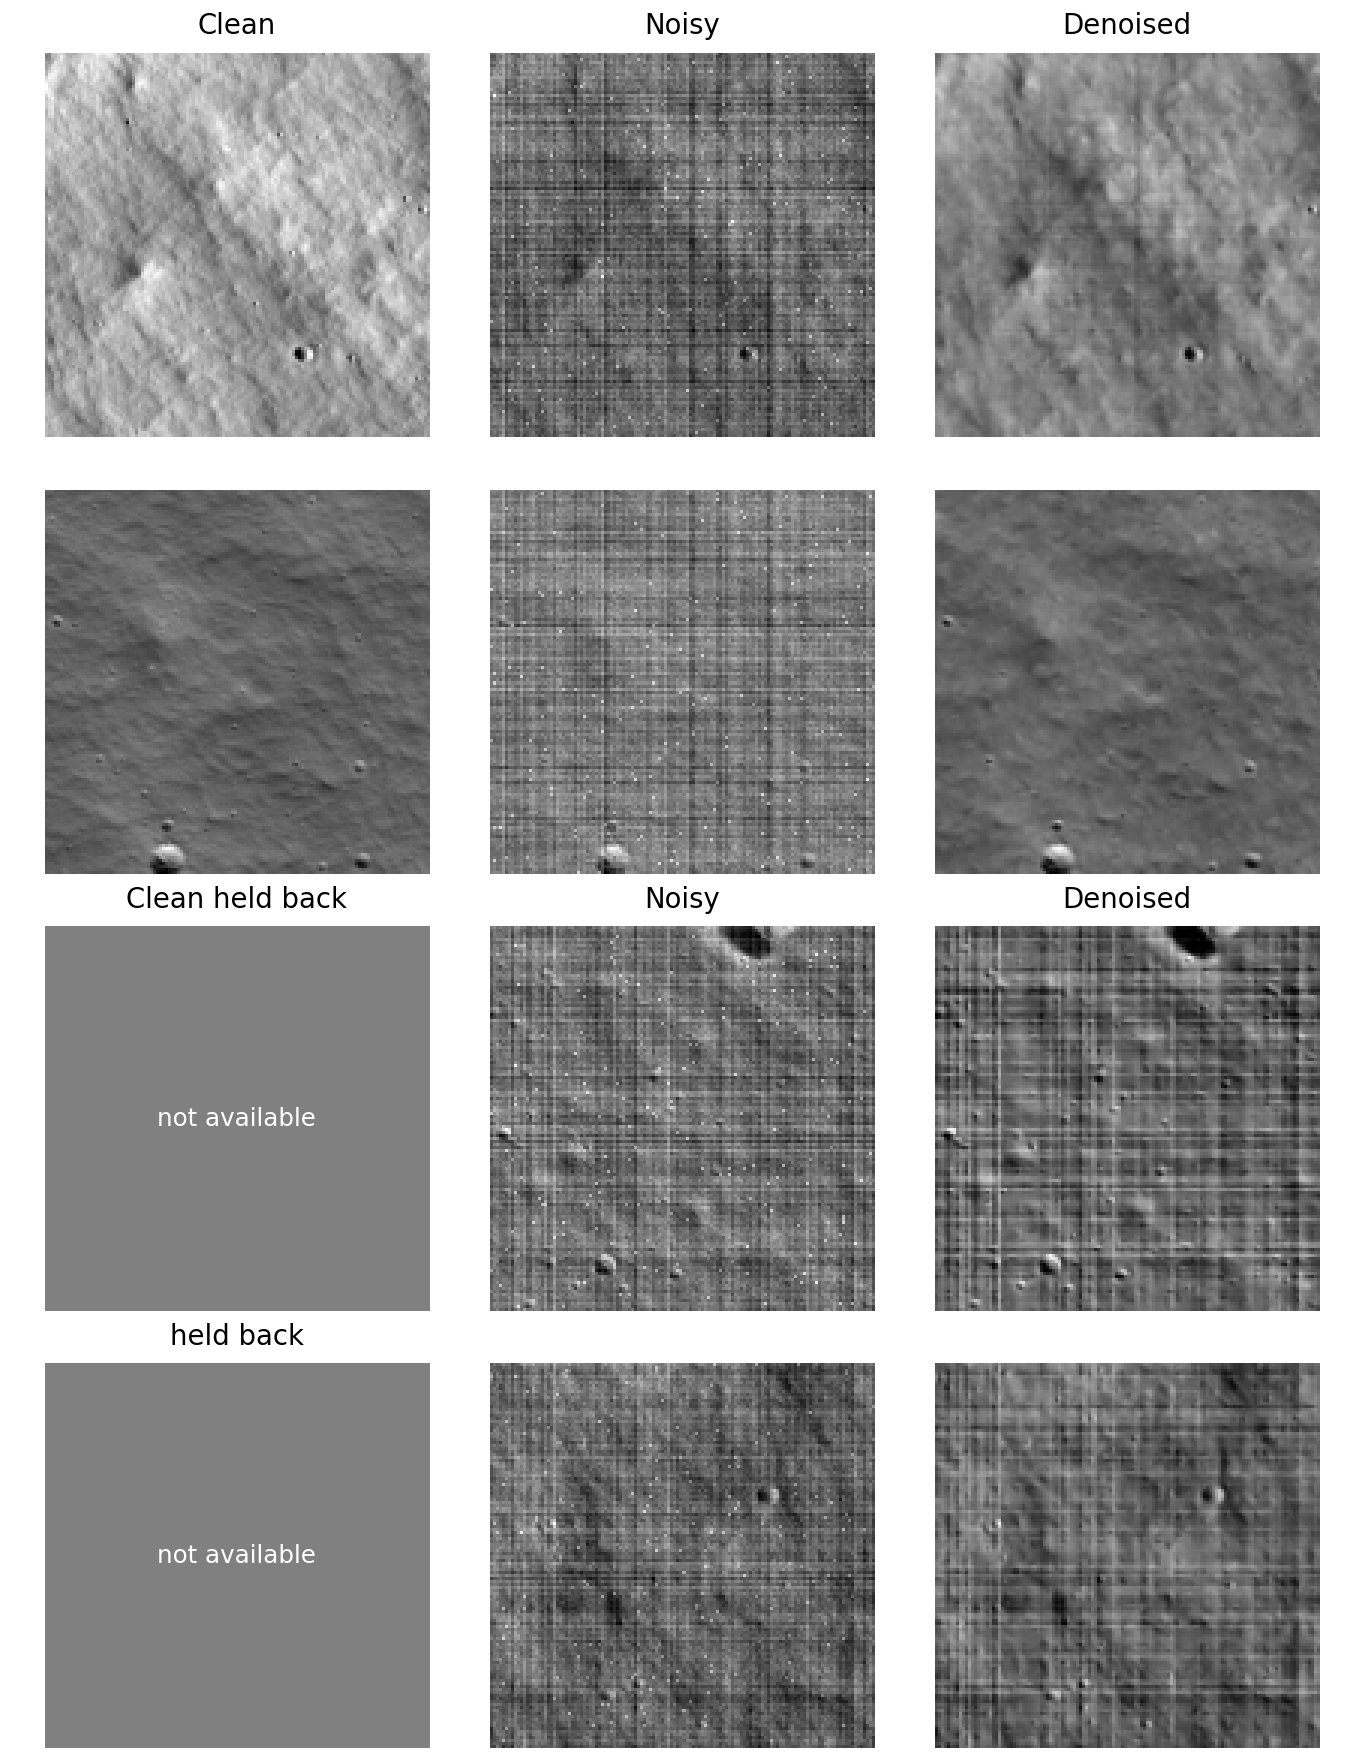
\includegraphics[width=0.82\textwidth]{images/final_visual_examples.png}
\caption{Two paired training examples and two blind-test examples. For blind-test images, the clean targets are held back by the assignment. The final Deep U-Net removes most high-frequency noise while preserving the dominant crater structures; some very fine contrast is still smoothed.} \textcolor{red}{WE NEED TO ADD THE TWO BLIND TEST IMAGES (old one were shit)}
\end{figure}

\section{Discussion}
\subsection{Challenges}
The main challenge was balancing denoising strength against preservation of small-scale lunar texture. Larger models reduced validation MSE, but also increased the risk of overfitting during long runs. This was addressed with dropout, AdamW weight decay, cosine learning-rate scheduling, and validation checkpointing. The validation curves show small oscillations, which is expected for a relatively small validation subset, but no divergence or training instability was observed.

Architecturally, the flat ResNet and autoencoder baselines were less competitive because they lacked the same combination of multi-scale context and direct high-resolution skip features. Attention U-Nets were more expressive, but in this problem the gates did not improve the final score and may have suppressed faint but useful surface texture. Diffusion models were a valuable risk-taking direction and produced plausible denoised images, but validation and inference were slower and the final quantitative metrics remained below the feed-forward Deep U-Net.

The blind test set has no clean target, so true test MSE/PSNR cannot be computed locally. For this reason, final model selection was based on paired validation metrics and qualitative inspection of the denoised blind-test predictions.

\section{Conclusion}
The final submitted model is a large four-stage Deep U-Net trained with MSE and AdamW. It was selected because it achieved the best completed validation score, trained stably on Euler, and gave the best visual trade-off between removing noise and preserving lunar structure. The project also showed that systematic ablations followed by Optuna refinement were more effective than trying isolated complex models: the ablations identified Deep U-Nets as the strongest family, and Optuna refined the learning rate, regularization, activation, and batch size within that family.
\section*{Use of Generative AI}

Generative AI tools including ChatGPT-5.3, Copilot, and Claude were used during the preparation of this document for LaTeX formatting, drafting of text and coding. The final content has been carefully reviewed and validated by the authors.


\end{document}
